%%%%%%%%%%%%%%%%%%%%%%%%%%%%%%%%%%%%%%%%%
% Beamer Presentation
% LaTeX Template
% Version 1.0 (10/11/12)
%
% This template has been downloaded from:
% http://www.LaTeXTemplates.com
%
% License:
% CC BY-NC-SA 3.0 (http://creativecommons.org/licenses/by-nc-sa/3.0/)
%
%%%%%%%%%%%%%%%%%%%%%%%%%%%%%%%%%%%%%%%%%

%----------------------------------------------------------------------------------------
%	PACKAGES AND THEMES
%----------------------------------------------------------------------------------------

\documentclass{beamer}

\mode<presentation> {

% The Beamer class comes with a number of default slide themes
% which change the colors and layouts of slides. Below this is a list
% of all the themes, uncomment each in turn to see what they look like.

%\usetheme{default}
%\usetheme{AnnArbor}
%\usetheme{Antibes}
%\usetheme{Bergen}
%\usetheme{Berkeley}
%\usetheme{Berlin}
%\usetheme{Boadilla}
%\usetheme{CambridgeUS}
%\usetheme{Copenhagen}
%\usetheme{Darmstadt}
%\usetheme{Dresden}
%\usetheme{Frankfurt}
%\usetheme{Goettingen}
%\usetheme{Hannover}
%\usetheme{Ilmenau}
%\usetheme{JuanLesPins}
%\usetheme{Luebeck}
%\usetheme{Madrid}
%\usetheme{Malmoe}
%\usetheme{Marburg}
%\usetheme{Montpellier}
%\usetheme{PaloAlto}
%\usetheme{Pittsburgh}
%\usetheme{Rochester}
%\usetheme{Singapore}
%\usetheme{Szeged}
\usetheme{Warsaw}

% As well as themes, the Beamer class has a number of color themes
% for any slide theme. Uncomment each of these in turn to see how it
% changes the colors of your current slide theme.

%\usecolortheme{albatross}
%\usecolortheme{beaver}
%\usecolortheme{beetle}
%\usecolortheme{crane}
%\usecolortheme{dolphin}
%\usecolortheme{dove}
%\usecolortheme{fly}
%\usecolortheme{lily}
%\usecolortheme{orchid}
%\usecolortheme{rose}
%\usecolortheme{seagull}
%\usecolortheme{seahorse}
%\usecolortheme{whale}
%\usecolortheme{wolverine}

%\setbeamertemplate{footline} % To remove the footer line in all slides uncomment this line
%\setbeamertemplate{footline}[page number] % To replace the footer line in all slides with a simple slide count uncomment this line

\setbeamertemplate{navigation symbols}{} % To remove the navigation symbols from the bottom of all slides uncomment this line
}

\usepackage{graphicx} % Allows including images
\usepackage{booktabs} % Allows the use of \toprule, \midrule and \bottomrule in tables
\usepackage{tabularx}
\usepackage{hyperref}
\usepackage{siunitx}

\graphicspath{ {img/} }

\title[MAVRIC]{Team Iceman IPR for MAVRIC}
\author{
	Chad Condon 
	%\url{ccondon@uw.edu}
	\and
	Keenan Fejeran 
	%\url{kfejeran@uw.edu}
	\and
	Ben Foster 
	%\url{benf94@uw.edu}
	\and
	Caleb Horst 
	%\url{calebjh@uw.edu}
}
\institute[UWT]{Institute of technology\\University of Washington Tacoma}
\date{April 14, 2015}

\begin{document}

% Title Slide
\begin{frame}
	\titlepage
\end{frame}

% Table of contents slide. Probably won't need this.
\begin{frame}
	\frametitle{Overview}
	\tableofcontents
\end{frame}

% Schedule slide. Include the gantt chart that we made.
\begin{frame}
	\frametitle{Schedule}
	\begin{figure}
		\centering
		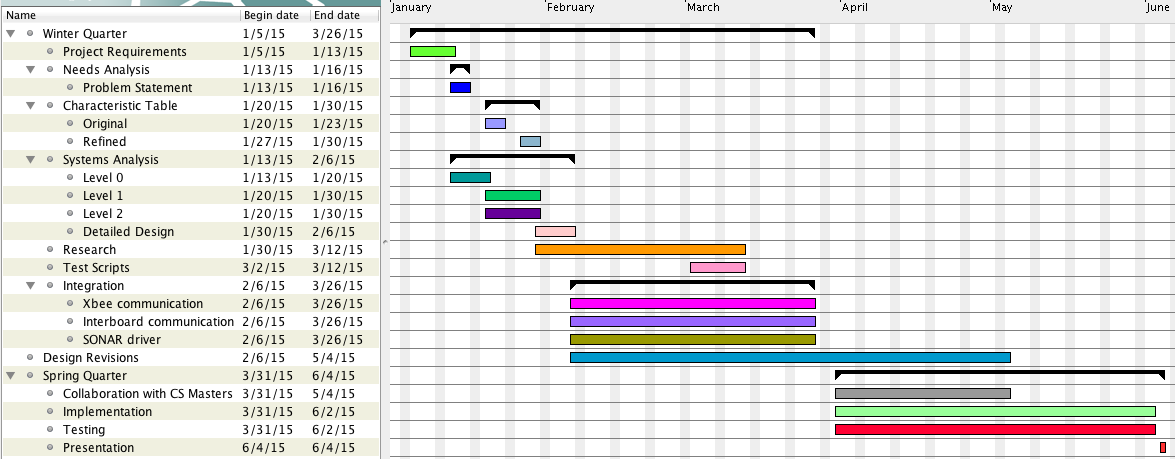
\includegraphics[width=\textwidth]{gantt.png}
	\end{figure}
\end{frame}

% Spec page. Include spec sheet?
\begin{frame}
	\frametitle{Specifications}
\end{frame}

% Needed parts. Pull from BOM?
\begin{frame}
	\frametitle{Parts Needed}
\end{frame}

% Bill of Materials page. Insert BOM
\begin{frame}
	\frametitle{Bill of Materials}
	\begin{table}
		\centering
		{\footnotesize
\begin{tabular}{llrrr}
                                                            &&                  & \textbf{Cost per}     &                       \\
    \multicolumn{2}{l}{\textbf{Item}}			& \textbf{Count}    & \textbf{Item}         & \textbf{Cost}         \\ \hline
    MAX4466 & electret microphone amplifier                 & 2                 & 16.00                 & 32.00                 \\
    MSGEQ7 & graphic equalizer display filter               & 2                 & 4.95                  & 9.90                  \\
    TM4C1294 LaunchPad & microcontroller board              & 1                 & 19.99                 & 19.99                 \\
    Raspberry Pi B+ & single board computer                 & 1                 & 29.99                 & 29.99                 \\
    ADXL335 & triple axis accelerometer                     & 1                 & 14.99                 & 14.99                 \\
    TSL235 & light-to-frequency converter                   & 3                 & ---                   & ---                   \\
    ATtiny85 & slave microcontroller                        & 1                 & ---                   & ---                   \\
    HC-SR04 & distance sensor                               & 1                 & 5.00                  & 5.00                  \\
    MCC7805 & \SI{5}{\volt} positive voltage regulator      & 1                 & ---                   & ---                   \\
    XBee Pro 900 RPSMA & wireless transceiver               & 2                 & ---                   & ---                   \\
    M891 & leaded NTC thermistor                            & 2                 & ---                   & ---                   \\
    ActivMedia Pioner 2 & chassis                           & 1                 & ---                   & ---                   \\
    PS-1270 & battery                                       & 2                 & ---                   & ---                   \\
    GM9236E132 & \SI{12}{\volt} DC motor                    & 2                 & ---                   & ---                   \\
    VNH5019A & motor controller                             & 2                 & ---                   & ---                   \\
    Wombat (PTH) & prototyping board                        & 4                 & 9.95                  & 39.80                 \\
    \multicolumn{2}{l}{Raspberry Pi Camera Board}           & 1                 & 25.00                 & 25.00                 \\
    FS7548 & flex sensor                                    & 4                 & 12.95                 & 51.80                 \\
    TIP122 & NPN Darlington transistor                      & 1                 & 0.66                  & 0.66                  \\
    \multicolumn{2}{l}{various resistors, capacitors, wire, etc.} & ---               & ---                   & ---                   \\ \hline
    \multicolumn{4}{r}{\textbf{Total}}                                                                  & 229.13                \\ \hline
\end{tabular}
Items without a cost are on hand.
}

	\end{table}
\end{frame}

% We could run the Robot Soccer Demo program.
\begin{frame}
	\frametitle{Demo?}
\end{frame}

% END FRAME
\begin{frame}
	\Huge{\centerline{Thank You} \centerline{Questions?}}
\end{frame}

\end{document}